\section{Type Analyzer}\label{sec:analyzer}

This section formally defines a modified $\ires$ and its type analysis
and presents a condition-based refinement of the type analysis to improve the analysis precision. 

\subsection{Intermediate Representation}\label{sec:ires}

\begin{figure}
  \centering
  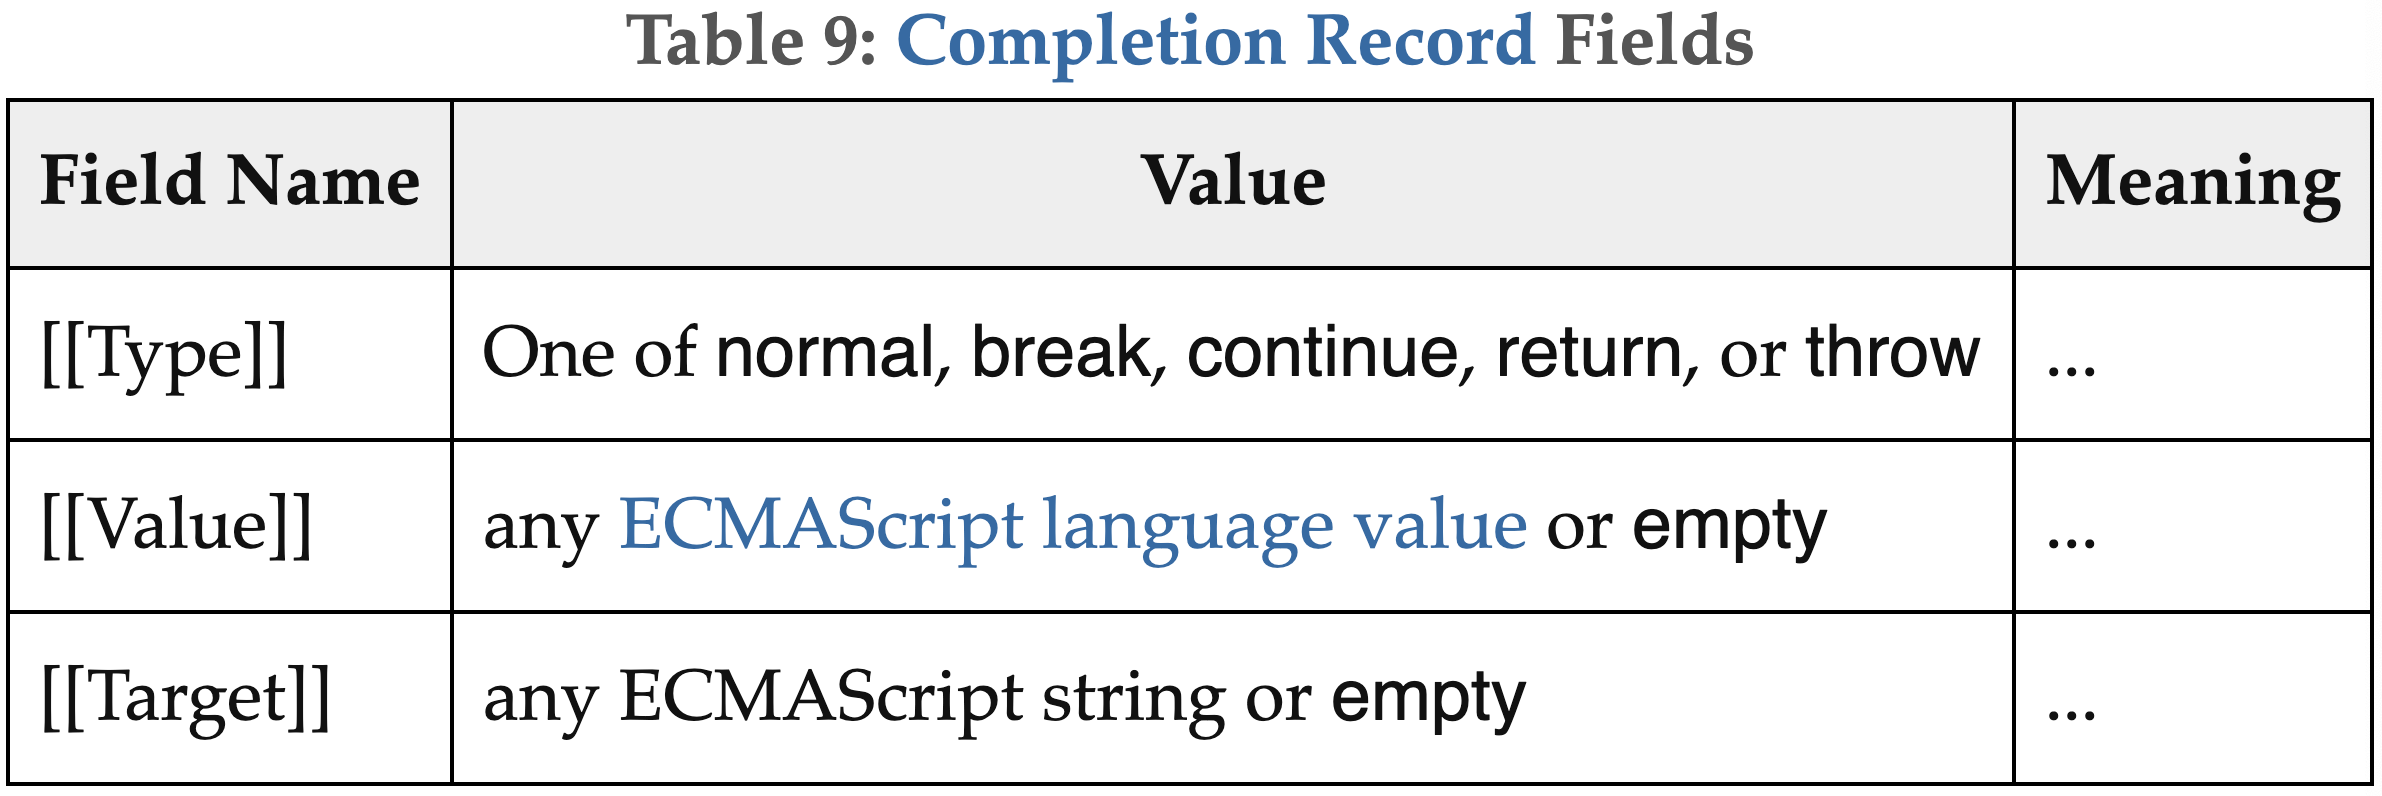
\includegraphics[width=0.48\textwidth]{img/record-fields-table}
  \caption{Fields of completion records in ECMAScript 2020}
  \label{fig:record-fields-table}
  \vspace*{-1.5em}
\end{figure}

$\ires$ is an untyped intermediate representation for ECMAScript~\cite{jiset}.
We modify it as a label-based language to make it suitable for type analysis as follows:
\begin{figure}[H]
  \centering
  \vspace*{-0.5em}
  \resizebox{\columnwidth}{!}{$
    \begin{array}{l@{~}r@{~}c@{~}r@{~}r@{~}l}
      \text{Functions}
      &\funcset&\ni&\func&::=&\kwdef \; \x (\x^*, \kwsl \x^* \kwsr). \; \lab\\

      \text{Instructions}
      &\instset&\ni&\inst&::=&
      \kwlet \; \x = \expr \mid
      \x = \kwrl \expr \; \expr^* \kwrr \mid
      \kwassert \; \expr \\

      &&&&\mid&
      \kwif \; \expr \; \lab \; \lab \mid
      \kwreturn \; \expr \mid
      \refer = \expr \\

      \text{References}
      &&&\refer&::=&
      \x \mid
      \refer \kwsl \expr \kwsr \\

      \text{Expressions}
      &&&\expr&::=&
      \tname \; \kwcl [\x: \expr]^* \kwcr \mid
      \clist{\expr^*} \mid
      \expr: \ty \mid
      \refer \kwexists \\

      &&&&\mid&
      \expr \bop \expr \mid
      \uop \; \expr \mid
      \refer \mid
      \const \mid
      \prim \\

      \text{Primitives}
      &\primset&\ni&\prim&::=&
      \undefval \mid \nullval \mid \bool \mid
      \num \mid \bigint \mid \str \mid \symb \\

      \text{Types} &\tyset&\ni&\ty&::=&\tname \mid \clist{} \mid \clist{\ty} \mid
      \tjs \mid \tprim\\

      &&&&\mid&
      \undefval \mid \nullval \mid \tbool \mid \tnumeric\\

      &&&&\mid&
      \tnum \mid \tbigint \mid \tstr \mid \tsymb \\
    \end{array}
  $}
  \vspace*{-0.5em}
\end{figure} \noindent
A modified $\ires$ program $\prog = (\getfunc, \getinst, \getnext)$ consists
of three mappings;  $\getfunc: \labset \rightarrow \funcset$
maps labels to their functions, $\getinst: \labset \rightarrow
\instset$ maps labels to their instructions, and $\getnext: \labset
\rightarrow \labset$ maps labels to their next labels, where a label $\lab \in \labset$
denotes a program point. A function $\kwdef \; \f (\x^*, \kwsl \y^* \kwsr). \;
\lab \in \funcset$ consists of its name $\f$, normal parameters $\x^*$, optional
parameters $\y^*$, and a body label $\lab$.  For presentation brevity,
we assume that no global variables exist in this paper.
An instruction $\inst$ is a variable declaration, a function call, an assertion,
a branch, a return, or a reference update.  An invocation of an abstract
algorithm in ECMAScript is compiled to a function call instruction with a new
temporary variable.  We represent loops using branch instructions with
cyclic pointing of labels in $\getnext$.  A reference $\refer$
is a variable $\x$ or a field access $\refer \kwsl \expr \kwsr$.  We write
$\refer.\f$ to briefly represent $\refer \kwsl \code{"f"} \kwsr$. An
expression $\expr$ is a record, a list, a type check, an existence check, a
binary operation, a unary operation, a reference, a constant, or a primitive,
which is either $\undefval$, $\nullval$, a \jscode{Boolean} $\bool$, a
\jscode{Number} $\num$, a \jscode{BigInt} $\bigint$, a \jscode{String} $\str$,
or a \jscode{Symbol} $\symb$.

\begin{figure}
  \centering
  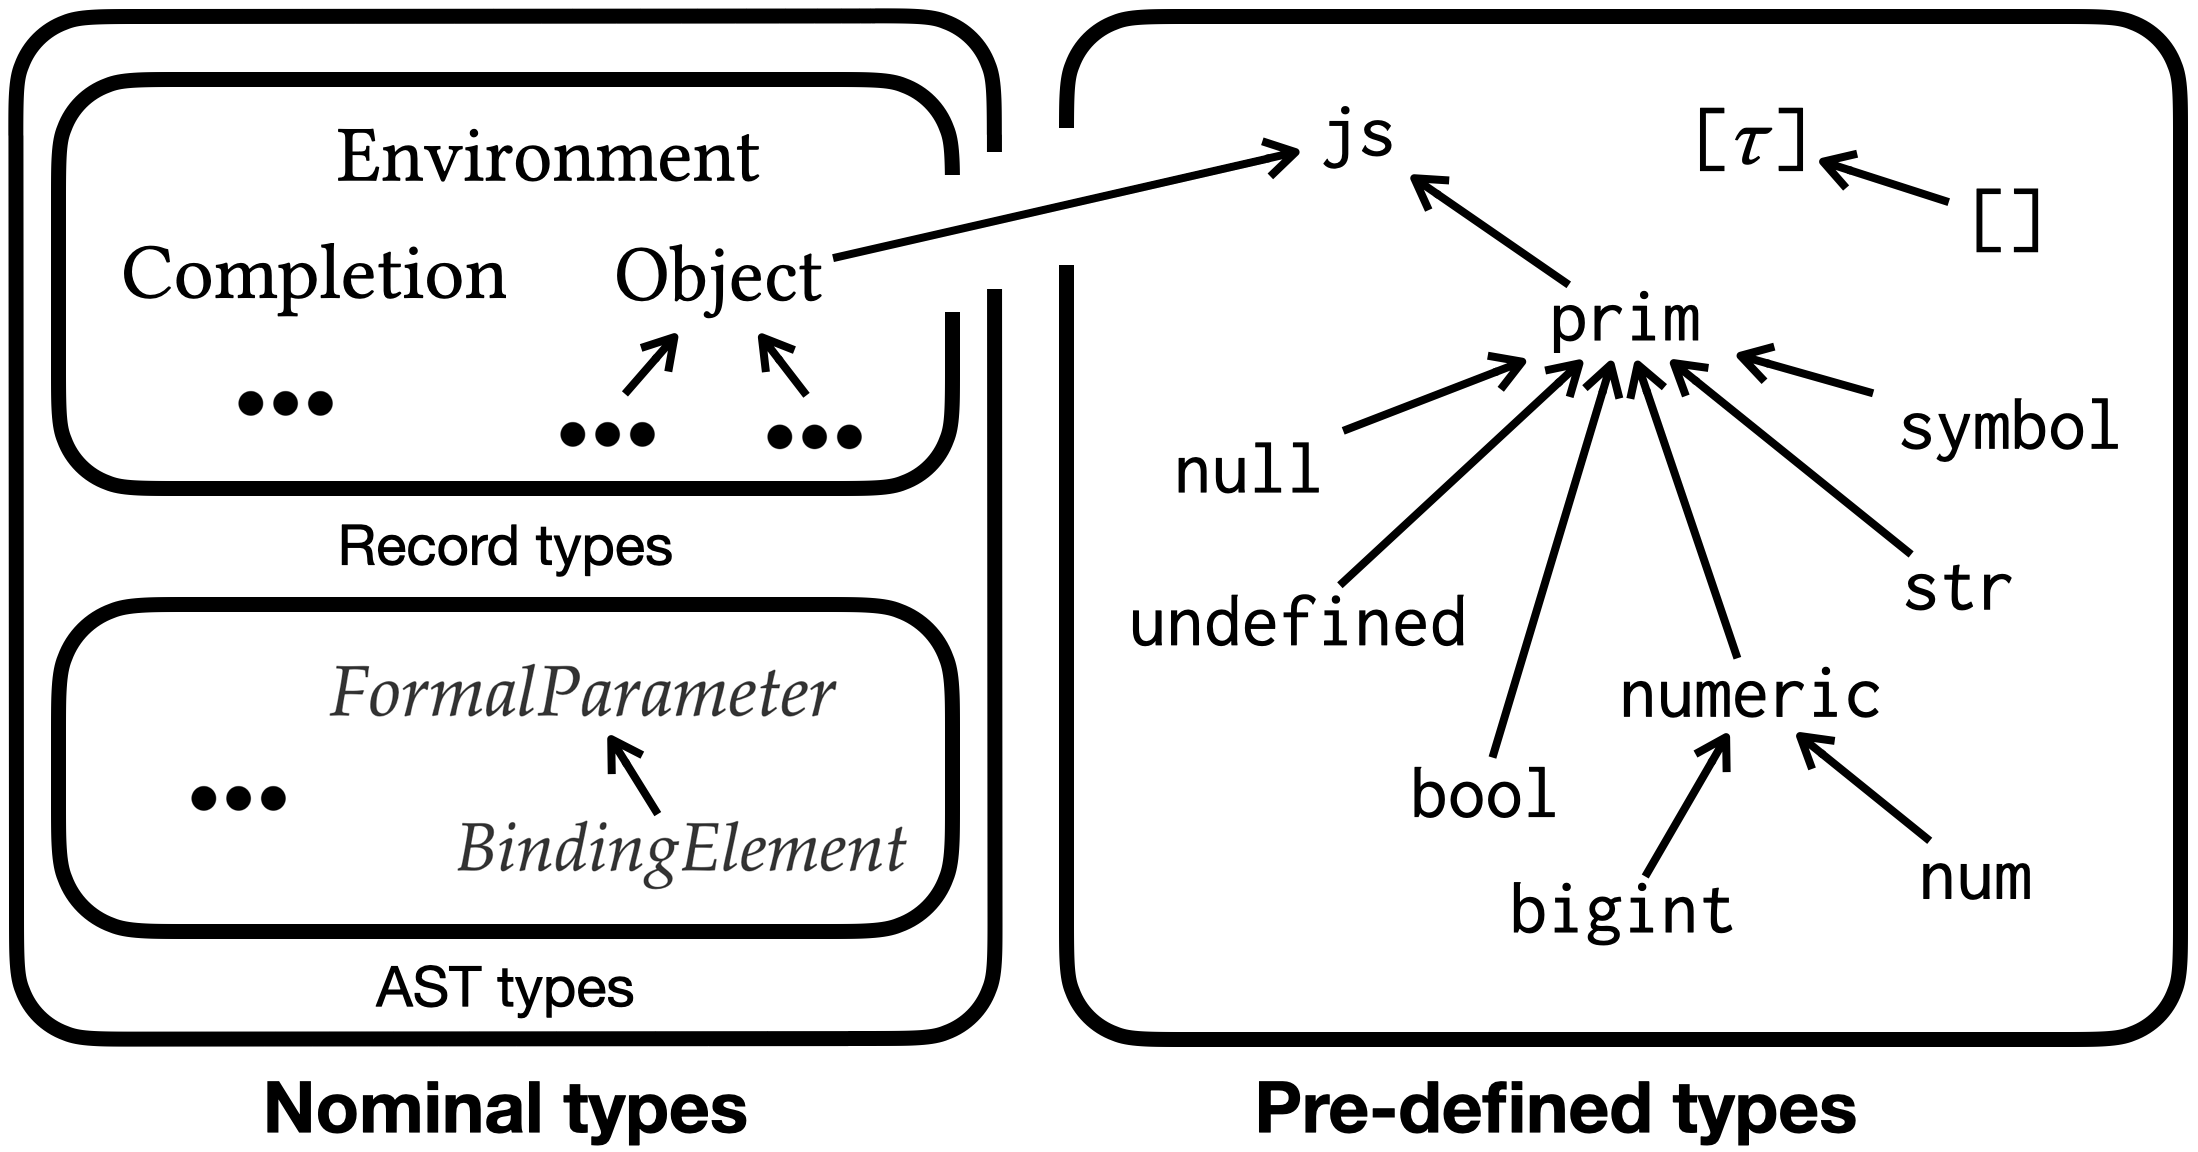
\includegraphics[width=0.4\textwidth]{img/subtype}
  \caption{A graphical representation of the subtype relation $\subtype$}
  \label{fig:subtype}
  \vspace*{-1.5em}
\end{figure}

\begin{figure*}[t]
  \centering
  \resizebox{0.49\textwidth}{!}{$
\renewcommand{\arraystretch}{1.3}
    \begin{array}{@{}l@{~}c@{~}l}
      \asemi{\kwlet \; \x = \expr}
      (\lab, \tys)(\aelem) &=&
      (\{ (\getnext(\lab), \tys) \mapsto \aenv[\x \mapsto
      \aseme{\expr}(\aenv)] \}, \emp)\\

      \asemi{\x = \kwrl \expr \; \expr_1 \cdots \expr_n \kwrr}
      (\lab, \tys)(\aelem) &=& (\rmap', \retp')\\
      \multicolumn{3}{@{}l}{
        \text{where} \;
        \left\{
          \begin{array}{l@{}}
            \aty = \aseme{\expr}(\aenv) \;\wedge\;
            \aty_1 = \aseme{\expr_1}(\aenv) \;\wedge\;
            \cdots \;\wedge\;
            \aty_n = \aseme{\expr_n}(\aenv) \;\wedge\;\\

            T' = \{ \upcasts([ \ty_1, \cdots, \ty_n ]) \mid \ty_1 \in \aty_1
            \;\wedge\; \cdots \;\wedge\; \ty_n \in \aty_n \} \;\wedge\;\\

            \func = \kwdef \; \f (\p_1, \cdots, \kwsl \cdots, \p_{m_\func}
            \kwsr). \; \lab_\func \;\wedge\;\\

            \aenv_{\func, \tys'} = [\p_1 \mapsto \{ \tys'[1] \}, \cdots,
            \p_{m_\func} \mapsto \{ \tys'[m] \}] \;\wedge\;\\

            \rmap' = \{ (\lab_\func, \tys') \mapsto \aenv_{\func, \tys'}
            \mid \func \in \aty \;\wedge\; \tys' \in T' \} \;\wedge\;\\

            \retp' = \{ (\func, \tys') \mapsto \{ (\getnext(\lab), \tys, \x)
            \} \mid \func \in \aty \;\wedge\; \tys' \in T' \}\\
          \end{array}
        \right.
      }\\
    \end{array}
  $}
  \resizebox{0.49\textwidth}{!}{$
\renewcommand{\arraystretch}{1.3}
    \begin{array}{@{}l@{~}c@{~}l}
      \asemi{\kwreturn \; \expr}
      (\lab, \tys)(\aelem) &=&
      (\{ (\lab_r, \tys_r) \mapsto \aenv_r \mid
      (\lab_r, \tys_r, \x) \in R\}, \emp)\\
      \multicolumn{3}{@{}l}{
        \text{where} \; R = \retp(\getfunc(\lab), \tys) \;\wedge\; \aenv_r =
        \rmap(\lab_r, \tys_r)[\x \mapsto \aseme{\expr}(\aenv)]
      }\\

      \asemi{\kwassert \; \expr}
      (\lab, \tys)(\aelem) &=&
      (\{ (\getnext(\lab), \tys) \mapsto \pass(\expr, \true)(\aenv) \}, \emp)\\

      \asemi{\kwif \; \expr \; \lab_\mt \; \lab_\mf}
      (\lab, \tys)(\aelem) &=&
      (\{ (\lab_\mt, \tys) \mapsto \pass(\expr, \true)(\aenv),\\ &&
      \phantom{(\{} (\lab_\mf, \tys) \mapsto \pass(\expr, \false)(\aenv) \}, \emp)\\

      \asemi{\x = \expr}
      (\lab, \tys)(\aelem) &=&
      (\{ (\getnext(\lab), \tys) \mapsto \aenv[\x \mapsto
      \aseme{\expr}(\aenv)] \}, \emp)\\

      \asemi{\refer \kwsl \expr_0 \kwsr = \expr_1}
      (\lab, \tys)(\aelem) &=&
      (\{ (\getnext(\lab), \tys) \mapsto \aenv \}, \emp)\\

      \multicolumn{3}{@{}l}{\text{where} \; \aelem = (\rmap, \retp) \;\wedge\;
      \aenv = \rmap(\lab, \tys)}
    \end{array}
  $}
\caption{Abstract semantics of instructions for a program $\prog = (\getfunc, \getinst, \getnext)$,
$\asemi{\inst}: (\labset \times \tyset^*) \rightarrow \adom \rightarrow \adom$
}
  \vspace*{-.5em}
  \label{fig:abs-sem}
\end{figure*}

A type $\ty \in \tyset$ is either a nominal type $\tname$, an empty list type
$\clist{}$, a parametric list type $\clist{\ty}$,
a JavaScript type $\tjs$,
a primitive type $\tprim$,
a numeric type $\tnumeric$,
$\tnum$, $\tbigint$, $\tstr$, or $\tsymb$.
A nominal type $\tname$ is either 1) an
\textit{AST type} with its corresponding syntax-directed algorithms as its fields,
or 2) a \textit{record type} with specific fields as described in ECMAScript.
For example, Figure~\ref{fig:record-fields-table} shows an excerpt from
ECMAScript 2020 (ES11) that describes the fields of completion records%
\footnote{https://262.ecma-international.org/11.0/\#table-8}, which we
model as follows:

\begin{figure}[H]
  \centering
  \vspace*{-0.5em}
  \resizebox{\columnwidth}{!}{$
    \begin{array}{l}
      \code{Completion} \code{=} \; \kwcl\\
        \quad \Type: \{ \nconst{normal}, \nconst{break}, \nconst{continue},
        \nconst{return}, \nconst{throw} \},\\
        \quad \Value: \{ \tjs, \nconst{empty} \},
        \quad \Target: \{ \tstr, \nconst{empty} \}\\
      \kwcr\\
    \end{array}
  $}
  \vspace*{-0.5em}
\end{figure}

The subtype relation $\subtype \subseteq \tyset \times \tyset$ between types is
depicted in Figure~\ref{fig:subtype}; a directed edge from $\ty'$ to $\ty$
denotes $\ty' \subtype \ty$ and the relation is reflexive and transitive.  The
subtype relation is dependent on the nominal types defined in ECMAScript.  We
extract the subtype relation for AST types from the JavaScript syntax.
For example, consider the syntax-directed abstract
algorithm at the lower-right part in Figure~\ref{fig:example}.
Because the nonterminal \textit{BindingElement} is the unique alternative of the
\textit{FormalParameter} production, we automatically extract the subtype
relation: \textit{BindingElement} $\subtype$ \textit{FormalParameter}. Using
the subtype relation, the expression $\expr: \ty$ checks whether the
evaluation result of $\expr$ has type $\ty'$ satisfying $\ty' \subtype \ty$.

We define a denotational semantics of the modified $\ires$ for instructions
$\semi{\inst}: \dom \rightarrow \dom$, references $\semr{\refer}: \dom
\rightarrow \valset$, and expressions $\seme{\expr}: \dom \rightarrow \valset$
where $\dom$ and $\valset$ denote states and values, respectively.
For brevity, we omit it in this paper and refer the
interested readers to a companion report~\cite{report}.


\subsection{Type Analysis}\label{sec:analysis}

We design a type analysis for the modified $\ires$ based on the abstract
interpretation framework~\cite{ai1977, ai1992} with analysis
sensitivity~\cite{sens-toplas}.  We first extend types as follows:
\begin{figure}[H]
  \centering
  \vspace*{-0.5em}
  \resizebox{0.8\columnwidth}{!}{$
    \tyset \ni \ty ::=
    \cdots \mid
    \func \mid
    \const \mid
    \bool \mid
    \str \mid
    \tabsent \mid
    \tnormal(\ty) \mid
    \tabrupt
  $}
  \vspace*{-0.5em}
\end{figure} \noindent
We add types for functions $\func$ and constants $\const$,
\jscode{Boolean} values $\bool$ and \jscode{String} values $\str$ to precisely
handle the control flows of branches and field accesses, respectively,
the absent type $\tabsent$ to represent the absence of variables, and
$\tnormal(\ty)$ for normal completions whose \code{Value} fields have
type $\ty$ and $\tabrupt$ for abrupt completions to enhance the
analysis precision.


Using the extended types, we define abstract states with flow-sensitivity and
type-sensitivity for arguments:

\begin{figure}[H]
  \centering
  \vspace*{-0.5em}
  \resizebox{\columnwidth}{!}{$
    \begin{array}{lr@{~}c@{~}c@{~}r@{~}l}
      \text{Abstract States}
      &\aelem&\in&\adom&=& \rmapset \times \retpset\\

      \text{Result Maps}
      &\rmap&\in&\rmapset&=& \labset \times \tyset^* \rightarrow \aenvset\\

      \text{Return Point Maps}
      &\retp&\in&\retpset&=& \funcset \times \tyset^*
      \rightarrow \partsof{\labset \times \tyset^* \times \varset} \\

      \text{Abstract Environments}
      &\aenv&\in&\aenvset&=&\varset \rightarrow \atyset\\

      \text{Abstract Types}
      &\aty&\in&\atyset&=&\partsof{\tyset}\\
    \end{array}
  $}
  \vspace*{-0.5em}
\end{figure}
\noindent
An abstract state $\aelem \in \adom$ is a pair of a result map and a return
point map.  A result map $\rmap \in \rmapset$ represents an abstract
environment for each flow- and type-sensitive view, and a return point map
$\retp \in \retpset$ represents possible return points of each function
with a type-sensitive context; each return point consists of a view for the
caller function and a variable that represents the return value.  An abstract
environment $\aenv \in \aenvset$ represents possible types for variables, and
$\aenv(\x) = \{ \tabsent \}$ when $\x$ is not defined in $\aenv$.  An abstract
type $\aty \in \atyset$ is a set of types.  We define the join operator
$\join$, the meet operator $\meet$, and the partial order $\order$ for most of
abstract domains in a point-wise manner, and define the operators for types with
a normalization function $\norm$ because of their subtype relations:
\begin{figure}[H]
  \centering
  \vspace*{-0.5em}
  \resizebox{\columnwidth}{!}{$
    \begin{array}{l}
      \aty_0 \join \aty_1 = \norm(\aty_0 \cup \aty_1)\\
      \aty_0 \meet \aty_1 = \norm(
      \{\ty_0 \in \aty_0 \mid \{ \ty_0 \} \order \aty_1 \} \cup
      \{\ty_1 \in \aty_1 \mid \{ \ty_1 \} \order \aty_0 \}
      )\\
      \aty_0 \order \aty_1 \Leftrightarrow \forall \ty_0 \in \aty_0. \; \exists
      \ty_1 \in \norm(\aty_1). \; \text{s.t.} \; \ty_0 \subtype \ty_1\\
    \end{array}
  $}
  \vspace*{-0.5em}
\end{figure} \noindent
where $\small{\norm(\aty) = \{ \ty \mid \ty \in \aty \wedge \nexists \ty' \in
\aty\setminus \{ \ty \}. \; \text{s.t.} \; \ty \subtype \ty' \}}$.

We now define the abstract semantics of instructions $\asemi{\inst}$ in Figure~\ref{fig:abs-sem}
and the abstract semantics of references $\asemr{\refer}$
and expressions $\aseme{\expr}$ in a companion report~\cite{report}.
To avoid the explosion of type-sensitive
views, we upcast the argument type before function calls with the
following function:
\begin{figure}[H]
  \centering
  \vspace*{-0.5em}
  \resizebox{0.8\columnwidth}{!}{$
    \upcast(\ty) = \left\{
      \begin{array}{ll}
        \tnormal(\upcast(\ty')) & \text{if} \; \ty = \tnormal(\ty')\\
        \clist{\upcast(\ty')} & \text{if} \; \ty = \clist{\ty'}\\
        \tstr & \text{if} \; \ty = \str\\
        \tbool & \text{if} \; \ty = \bool\\
        \ty & \text{otherwise}\\
      \end{array}
    \right.
  $}
  \vspace*{-0.5em}
\end{figure} \noindent
and $\upcasts$ denotes a point-wise extension of $\upcast$ for type sequences.
For branches and assertions, we use the following $\pass$ function to prevent
infeasible control flows:

\begin{figure}[H]
  \centering
  \vspace*{-0.5em}
  \resizebox{0.9\columnwidth}{!}{$
    \pass(\expr, \bool)(\aenv) = \left\{
      \begin{array}{ll}
        \refine(\expr, \bool)(\aenv)
        & \text{if} \; \{ \true \} \order \aseme{\expr}(\aenv)\\

        \emp
        & \text{otherwise}\\
      \end{array}
    \right.
  $}
  \vspace*{-0.5em}
\end{figure} \noindent
where $\refine$ prunes out infeasible parts in abstract
environments using their conditions as we describe in Section~\ref{sec:refine}.
Then, we define the abstract
semantics $\asem{\prog}$ of a program $\prog$
as the least fixpoint of the abstract transfer $\atransfer: \adom \rightarrow
\adom$:
\begin{figure}[H]
  \centering
  \vspace*{-0.5em}
  \resizebox{0.9\columnwidth}{!}{$
    \begin{array}{r@{~}c@{~}l}
      \asem{\prog} &=& \lim_{n \rightarrow \infty}(\atransfer)^n(\iaelem)\\
      \atransfer(\aelem) &=& \aelem \join \left(
        \bigjoin_{(\lab, \tys) \in \domain{\rmap}}
        \asemi{\getinst(\lab)}(\lab, \tys)(\aelem)
      \right)\\
    \end{array}
  $}
  \vspace*{-0.5em}
\end{figure} \noindent
where $\aelem = (\rmap, \_)$ and $\iaelem$ denotes the initial abstract state.
As described in Section~\ref{sec:overview}, $\iaelem$ contains the entry points of
all syntax-directed algorithms without additional parameters and built-in
algorithms with appropriate abstract environments.
For a syntax-directed algorithm, we construct its abstract environment containing the variable
$\this$ with its production type and other variables for nonterminals.
For example, the upper-left syntax-directed algorithm in Figure~\ref{fig:example} is
initialized with the following abstract environment:
\begin{figure}[H]
  \centering
  \vspace*{-0.5em}
  \resizebox{\columnwidth}{!}{$
    \begin{array}{r@{~}c@{~}l}
      \this &\mapsto& \{ \code{AssignmentExpression} \},\\
      \code{LeftHandSideExpression} &\mapsto& \{ \code{LeftHandSideExpression} \},\\
      \code{AssignmentExpression} &\mapsto& \{ \code{AssignmentExpression} \}
    \end{array}
  $}
  \vspace*{-0.5em}
\end{figure} \noindent
For built-in algorithms, we assign pre-defined variables $\this$, $\args$, and
$\NewTarget$ with their corresponding types and parameters with $\tjs$ types.  For
example, the following abstract environment is for the built-in
algorithm $\jscode{Math.round}$ at the upper-right part in Figure~\ref{fig:example}:
\begin{figure}[H]
  \centering
  \vspace*{-0.5em}
  \resizebox{0.9\columnwidth}{!}{$
    \begin{array}{r@{~}c@{~}lr@{~}c@{~}l}
      \this &\mapsto& \{ \tjs \}, &
      \args &\mapsto& \{ \clist{\tjs} \},\\
      \NewTarget &\mapsto& \{ \code{Object}, \undefval \}, &
      \x &\mapsto& \{ \tjs \}\\
    \end{array}
  $}
  \vspace*{-0.5em}
\end{figure}


\subsection{Condition-based Refinement}\label{sec:refine}

We present a \textit{condition-based refinement} of the type analysis for the
modified $\ires$ to enhance the analysis precision.  It prunes out infeasible parts
in abstract environments using the conditions of branches and assertions.
We formally define the $\refine$ function as follows:
\begin{figure}[H]
  \centering
  \vspace*{-0.5em}
  \resizebox{\columnwidth}{!}{$
    \begin{array}{@{}r@{~}c@{~}l@{}}
      \refine(\code{!} \expr, \bool)(\aenv) &=&
      \refine(\expr, \neg \bool)(\aenv)\\

      \refine(\expr_0 \; \code{||} \; \expr_1, \bool)(\aenv) &=&
      \left\{
        \begin{array}{ll}
          \aenv_0 \join \aenv_1 & \text{if} \; \bool\\
          \aenv_0 \meet \aenv_1 & \text{if} \; \neg\bool\\
        \end{array}
      \right.\\
      \refine(\expr_0 \; \code{\&\&} \; \expr_1, \bool)(\aenv) &=&
      \left\{
        \begin{array}{ll}
          \aenv_0 \meet \aenv_1 & \text{if} \; \bool\\
          \aenv_0 \join \aenv_1 & \text{if} \; \neg\bool\\
        \end{array}
      \right.\\

      \refine(\x.\Type \; \code{==} \; \nconst{normal}, \true)(\aenv) &=&
      \aenv[ \x \mapsto \aty_\x \cap \tnormal(\tyset) ]\\
      \refine(\x.\Type \; \code{==} \; \nconst{normal}, \false)(\aenv) &=&
      \aenv[ \x \mapsto \aty_\x \cap \{ \tabrupt \} ]\\

      \refine(\x \; \code{==} \; \expr, \true)(\aenv) &=&
      \aenv[ \x \mapsto \aty_\x \meet \aty_\expr ]\\
      \refine(\x \; \code{==} \; \expr, \false)(\aenv) &=&
      \aenv[ \x \mapsto \aty_\x \setminus
      \lfloor\aty_\expr\rfloor ]\\

      \refine(\x : \ty, \true)(\aenv) &=&
      \aenv[ \x \mapsto \aty_\x \meet \{ \ty \} ]\\
      \refine(\x : \ty, \false)(\aenv) &=&
      \aenv[ \x \mapsto \aty_\x \setminus \{ \ty' \mid \ty' \subtype \ty
      \}]\\
      \refine(\expr, \bool)(\aenv) &=& \aenv\\
    \end{array}
  $}
  \vspace*{-0.5em}
\end{figure} \noindent
where $\aenv_j = \refine(\expr_j, \bool)(\aenv)$ for $j = 0, 1$,
$\aty_\expr = \aseme{\expr}(\aenv)$, and $\getSingle{\aty}$
returns $\{ \ty \}$ if $\aty$ denotes a singleton type $\ty$, or
returns $\emp$, otherwise.
